\documentclass{article}
\usepackage[T1]{fontenc}
\usepackage[utf8]{inputenc}
\usepackage{url}
\usepackage{amsmath}
\usepackage{hyperref}
\usepackage{graphicx}
\usepackage{natbib}
\usepackage[italian]{babel}
%\usepackage{babelbib}
\title{Come emettere una moneta digitale di banca centrale}
\author{David Chaum\footnote{david@chaum.com} \\
  xx Network \and
  Christian Grothoff\footnote{christian.grothoff@bfh.ch} \\
  BFH\footnote{Università di Scienze Applicate di Berna}
  \ e Progetto GNU \and
  Thomas Moser\footnote{thomas.moser@snb.ch} \\
  Banca Nazionale Svizzera}
\date{Questa versione: febbraio 2022 \\
      Prima versione:  maggio 2020}

\addto\captionsitalian{\renewcommand{\figurename}{Diagramma}}
\hyphenation{CBDC,Allen,Ni\-co\-las,Meikle\-john,Nie\-pelt}

\begin{document}

\maketitle

\begin{abstract}
Con l'emergere di Bitcoin e delle criptovalute stabili (per es. Diem,
già nota come Libra) recentemente proposte dai colossi del web, le
banche centrali affrontano una crescente concorrenza da parte di
operatori privati che offrono la propria alternativa digitale al
contante fisico. Non trattiamo qui la questione normativa se una banca
centrale debba emettere o meno una moneta digitale. Contribuiamo invece
all'attuale dibattito di ricerca spiegando in che modo una banca centrale
potrebbe farlo, se lo volesse. Proponiamo un sistema basato su token
senza tecnologia di registro distribuito, e mostriamo che le monete
elettroniche emesse in passato, basate solo su software, possono essere
migliorate per tutelare la privacy nelle transazioni, soddisfare i
requisiti normativi in modo efficace e offrire un livello di protezione
resistente ai computer quantistici contro il rischio sistemico per
la privacy. Né la politica monetaria né la stabilità del sistema
finanziario sarebbero realmente interessate da questo sistema dal
momento che una CBDC emessa in questo modo replicherebbe il contante
fisico anziché i depositi bancari. \\

JEL: E42, E51, E52, E58, G2
\\

Parole chiave: monete digitali, banca centrale, CBDC, firma cieca,
criptovalute stabili, \textit{stablecoins}
\end{abstract}

\vspace{40pt}

\section*{Ringraziamenti}
Vorremmo ringraziare Michael Barczay, Roman Baumann, Morten Bech,
Nicolas Cuche, Florian Dold, Andreas Fuster, Stefan Kügel, Benjamin
Müller, Dirk Niepelt, Oliver Sigrist, Richard Stallman, Andreas Wehrli
e tre collaboratori anonimi per i loro commenti e suggerimenti. Le
posizioni, le opinioni, i risultati e le conclusioni o raccomandazioni
espresse in questo documento sono strettamente quelle degli autori.
Non riflettono necessariamente le posizioni della Banca nazionale
svizzera (BNS). La BNS declina ogni responsabilità per eventuali
errori, omissioni o inesattezze che dovessero comparire nel documento.

Traduzione: Dora Scilipoti, con contributi da Luca Saiu
\newpage

%\tableofcontents

%\bibpunct{(}{)}{ e }{a}{}{,}

\section{Introduzione}\label{1.-introduzione}

Dall'avvento dei personal computer negli anni ottanta, e più
specificamente da quando nel 1991 la \textit{National Science
Foundation} revocò le restrizioni sull'uso di Internet per scopi
commerciali, c'è stata una ricerca sulla creazione di moneta digitale
per i pagamenti online. La prima proposta è stata quella
di~\cite{Chaum1983}. Sebbene tali metodi siano stati attuati, non hanno
preso piede; le carte di credito sono invece diventate il metodo più
diffuso per i pagamenti online. La proposta di~\cite{Nakamoto} per una
versione puramente \textit{peer-to-peer} di moneta digitale e il
conseguente lancio di Bitcoin avvenuto con successo hanno inaugurato
una nuova era di ricerca e sviluppo di valute digitali. La piattaforma
CoinMarketCap elenca oltre 5.000 criptovalute. Recentemente le banche
centrali hanno iniziato a considerare, o almeno a studiare,
l'emissione di monete digitali~\cite[vedi][]{AuerBoehme,AuerCornelli,Boar,Kiff,Mancini-Griffoli}.

Attualmente le banche centrali emettono due tipi di moneta: (i)
riserve sotto forma di conti di regolamento presso le banche centrali,
destinate solo agli operatori dei mercati finanziari, e (ii) divisa
disponibile per tutti sotto forma di banconote. Di conseguenza, la
letteratura sulla moneta digitale di banca centrale (\textit{Central Bank
Digital Currency} - CBDC) distingue tra (a) CBDC all'ingrosso ad
accesso ristretto e (b) CBDC al dettaglio disponibile per il
pubblico~\cite[si veda, ad esempio,][]{Bech}.
Una CBDC all'ingrosso sarebbe meno destabilizzante per il sistema attuale
dato che le banche e gli operatori dei mercati finanziari hanno già
accesso alla moneta digitale della banca centrale sotto forma di conti
presso questa istituzione, che utilizzano per regolare i pagamenti
interbancari. La domanda qui è se la tokenizzazione della moneta di banca
centrale e la tecnologia di registro distribuito (\textit{Distributed Ledger
Technology} - DLT) offrano vantaggi particolari rispetto ai sistemi con
regolamento lordo in tempo reale (\textit{Real-Time Gross Settlement} - RTGS)
esistenti. Finora la risposta è negativa, almeno per i pagamenti
interbancari nazionali~\cite[vedi][]{Chapman}.

Una CBDC al dettaglio, che sarebbe una nuova forma di moneta di banca
centrale disponibile per il pubblico, potrebbe essere più destabilizzante
per il sistema attuale, a seconda di come è progettata. Più una CBDC
compete con i depositi delle banche commerciali, maggiore è la minaccia
ai finanziamenti bancari, con effetti potenzialmente negativi sul credito
bancario e sull'attività economica~\cite[vedi][]{Agur}. Tuttavia, una
CBDC al dettaglio potrebbe anche essere
vantaggiosa~\cite[vedi][]{Bordo,Berentsen,Bindseil,Niepelt,Riksbank,BoE}.
Mettere a disposizione di tutti una moneta elettronica di banca centrale
esente dal rischio di controparte potrebbe migliorare la stabilità e la
resilienza del sistema di pagamenti al dettaglio. Potrebbe inoltre fornire
un'infrastruttura di pagamento neutrale per incoraggiare la concorrenza,
l'efficienza e l'innovazione. Nel complesso, è probabile che i costi e i
benefici di una CBDC al dettaglio differiscano da un paese all'altro. Per
il punto di vista della Banca nazionale svizzera, che non ha in programma
l'emissione di una CBDC al dettaglio, si veda~\cite{Jordan}.

Nel presente documento analizziamo la CBDC al dettaglio, ma senza
affrontare la questione se una banca centrale \emph{debba o meno} emetterla.
Ci concentriamo invece sul possibile design di una CBCD. L'interesse
per la progettazione di CBDC è recentemente aumentato
considerevolmente (si veda, ad esempio, ~\cite{Allen} e \cite{BoE}). Il design che
proponiamo differisce notevolmente da altre proposte. Il nostro sistema
si basa sulla tecnologia eCash descritta da~\cite{Chaum1983} e \cite{Chaum1990},
migliorandola. In particolare, proponiamo una CBDC basata su token, solo
con software e senza tecnologia di registro distribuito. La DLT è
un'architettura interessante in assenza di un operatore centrale o se le
entità che interagiscono non accettano di nominare un operatore centrale
fidato. Questo non è certo il caso di una CBDC al dettaglio emessa da una
\emph{banca centrale}. Distribuire il registro delle transazioni della
banca centrale con una \textit{blockchain} non fa che aumentare i costi
di transazione; non porta alcun vantaggio tangibile nell'implementazione
da parte di una banca centrale. L'utilizzo della DLT per emettere moneta
digitale può essere utile in assenza di una banca centrale (ad esempio,
il progetto Sovereign delle Isole Marshall) o se l'intenzione esplicita
è quella di fare a meno di una banca centrale (ad esempio,
Bitcoin).\footnote{Potrebbero esserci casi opportuni di utilizzo della
DLT per le infrastrutture dei mercati finanziari, come gli scambi digitali,
dove sorge la questione di come incorporare la moneta della banca centrale
all'interno di una struttura DLT per eseguire i regolamenti. Tuttavia,
in tali situazioni i potenziali benefici della DLT, ad esempio costi
inferiori o riconciliazione automatica, non derivano da un'emissione
decentralizzata di moneta di banca centrale.}

La CBDC basata su token che proponiamo consente anche di preservare
una caratteristica fondamentale del contante fisico: la privacy nelle
transazioni. Spesso si sostiene che l'uso della crittografia per la
tutela della privacy richieda così tanta potenza di calcolo da rendere
impraticabile la sua implementazione su dispositivi
portatili~\cite[vedi][]{Allen}. Sebbene questo possa essere vero nel
caso di una tecnologia di registro distribuito, dove la tracciabilità
delle transazioni è necessaria per prevenire la doppia spesa~\cite[][]{Narayanan},
non lo è nel caso proposto in questo documento, dove si ha un protocollo
di firma cieca di tipo Chaum e la partecipazione di una banca centrale.
La nostra CBDC, basata su firme cieche e un'architettura a due livelli,
garantisce una tutela della privacy nelle transazioni perfetta e
quanto-resistente, fornendo al contempo protezioni sociali che sono di
fatto più potenti rispetto a quelle delle banconote per la lotta al
riciclaggio di denaro (\textit{Anti-Money Laundering} - AML) e al
finanziamento del terrorismo (\textit{Counter Terrorism Financing} - CFT).

La privacy nelle transazioni è importante per tre motivi. In primo luogo,
protegge gli utenti dal potenziale abuso di monitoraggio e sorveglianza
da parte dei governi. Anche se si pensa di non avere nulla da nascondere,
i piani di sorveglianza di massa restano problematici, se non altro per
il rischio di errori e abusi, soprattutto se condotti senza trasparenza
e responsabilità~\cite[vedi][]{Solove}. In secondo luogo, la privacy nelle
transazioni protegge gli utenti dallo sfruttamento dei dati da parte dei
fornitori di servizi di pagamento. Infine, salvaguarda gli utenti dalla
controparte nelle transazioni in quanto esclude possibili comportamenti
opportunistici successivi o rischi per la sicurezza dovuti a negligenza
o mancata protezione dei dati dei clienti~\cite[vedi][]{Kahn2005}.

Questo documento è strutturato come segue: nella Sezione II si spiega
la differenza tra la moneta di banca centrale e altri tipi di moneta.
Nella Sezione III si esaminano i modelli di CBDC tipici e generici prima
di proporre il nostro progetto nella Sezione IV. Si considerano poi
gli aspetti normativi e le politiche (V) e il relativo lavoro (VI).
Infine, si conclude (VII).


\section{Cos'è la moneta di banca centrale?}
        \label{2.-cos'è-la-moneta-di-banca-centrale}

La moneta è un attivo che può essere utilizzato per acquistare beni e
servizi. Per essere considerato moneta, l'attivo deve essere accettato
da entità diverse dall'emittente. Ecco perché i voucher, ad esempio,
non sono considerati moneta. La moneta autentica deve essere
\emph{comunemente} accettata come mezzo di scambio. Sebbene la moneta
abbia altre funzioni, ad esempio come unità di conto e riserva di valore,
la sua caratteristica distintiva è la sua funzione di mezzo di scambio.
Normalmente l'unità di conto (cioè come avvengono la fissazione dei
prezzi e la contabilizzazione dei debiti) coincide per ragioni
pratiche con il mezzo di scambio. Una separazione può tuttavia
verificarsi se il valore del mezzo di scambio manca di stabilità
rispetto ai beni e servizi scambiati.\footnote{Ciò può accadere
spontaneamente in un ambito caratterizzato da un'inflazione elevata,
ad esempio quando i prezzi sono quotati in USD ma i pagamenti vengono
effettuati in valuta locale. Lo stesso vale per i pagamenti in Bitcoin,
dove i prezzi sono solitamente fissati in USD o altre valute locali a
causa dell'elevata volatilità del Bitcoin. Una separazione può anche
essere progettata appositamente, come nel caso
dell'\textit{Unidad de Fomento} (UF) in Cile o i Diritti Speciali di
Prelievo (DSP) del Fondo Monetario Internazionale (FMI). Tuttavia,
anche in questi casi lo scopo è quello di avere un'unità di conto più
stabile.} La moneta deve anche essere una riserva di valore per fungere
da mezzo di scambio perché deve preservare il suo potere d'acquisto tra
il momento in cui si riceve e quello in cui si spende. In ogni modo,
ci sono molti altri attivi che fungono da riserva di valore, come azioni,
obbligazioni, metalli preziosi e immobili. Pertanto, la caratteristica
di riserva di valore non è distintiva della moneta.

In un'economia moderna, il pubblico utilizza due tipi diversi di
moneta: (a) moneta statale e (b) moneta privata. La moneta statale viene
generalmente emessa dalla banca centrale, che agisce in qualità di
agente dello Stato. La moneta della banca centrale è disponibile per
alcune istituzioni finanziarie sotto forma di depositi presso la banca
centrale (riserve) e per il pubblico sotto forma di valuta (banconote e
monete), nota anche come «contante». In una economia moderna con valuta
fiat, tale moneta non ha un valore intrinseco. Legalmente è una passività
della banca centrale, sebbene non sia rimborsabile. Nella maggior parte
dei paesi, la moneta della banca centrale è definita come avente corso
legale, il che significa che deve essere accettata per il pagamento dei
debiti monetari, comprese le tasse e le sanzioni legali. Sebbene ciò
garantisca un certo valore alla moneta della banca centrale, lo status
di corso legale non è sufficiente per mantenere un valore stabile. È la
politica monetaria della banca centrale che mantiene il valore della
moneta. Mantenere la stabilità dei prezzi, vale a dire un valore stabile
della moneta rispetto a quello dei beni e dei servizi scambiati, è
infatti una delle principali responsabilità delle banche centrali.

La maggior parte dei pagamenti in un'economia moderna vengono effettuati
con moneta privata emessa dalle banche commerciali ed è costituita da
depositi bancari a vista che le persone detengono presso queste banche.
Sono depositi che si posssono utilizzare mediante assegni, carte di
debito, carte di credito e altri mezzi di trasferimento di denaro e
costituiscono una passività della banca commerciale di riferimento. Una
caratteristica fondamentale di questi depositi è che le banche commerciali
garantiscono la convertibilità su richiesta in moneta della banca centrale
ad un prezzo fisso, vale a dire, alla pari. I depositanti possono prelevare
i propri fondi in contante o trasferirli ad un valore fisso di 1:1. Le
banche commerciali mantengono stabile il valore della propria moneta
ancorandola a quella della banca centrale.

Tuttavia, in un sistema di riserva frazionaria, una banca commerciale,
anche se solvibile, potrebbe non avere liquidità a sufficienza per
onorare la sua promessa di convertire i depositi bancari in moneta
della banca centrale (ad esempio, nel caso di una corsa agli sportelli)
in modo tale che i clienti non possano prelevare i propri soldi. Una
banca può anche diventare insolvente e fallire, e di conseguenza i
clienti possono perdere denaro. Per questo motivo le banche commerciali
sono soggette a regolamentazioni volte a mitigare tali rischi.

Una differenza notevole tra la moneta di una banca centrale e la
moneta privata emessa da una banca commerciale è, pertanto, che
quest'ultima comporta un rischio di controparte. Una banca centrale
può sempre adempiere ai suoi obblighi utilizzando la propria moneta
non rimborsabile. In un'economia nazionale, la moneta della banca
centrale è l'unico attivo monetario esento da rischi di credito e di
liquidità. È pertanto l'attivo tipicamente preferito per regolare i
pagamenti nelle infrastrutture dei mercati finanziari (si veda, per
esempio, \textit{CPMI-IOSCO Principles for Financial Market
Infrastructures}, 2012). Un'altra differenza risiede nella capacità
della moneta della banca centrale di sostenere il sistema monetario
nazionale fornendo un valore di riferimento con cui la moneta delle
banche commerciali mantiene la piena convertibilità.

A parte le banche commerciali, altre entità private tentano
occasionalmente di emettere moneta; le criptovalute sono solo il
tentativo più recente. Ma a differenza dei depositi bancari, tale
moneta non è comunemente accettata come mezzo di scambio. Questo vale
anche per Bitcoin, la criptovaluta più ampiamente accettata. Un
ostacolo all'utilità delle criptovalute come mezzo di scambio è l'elevata
volatilità del loro valore. In risposta a questo problema sono emerse
le criptovalute stabili, cosiddette «stablecoins». Le
\textit{stablecoin} generalmente tentano di stabilizzare il proprio
valore in due modi: imitando le banche centrali (\textit{stablecoin}
algoritmiche) o imitando le banche commerciali e strumenti di
investimento (\textit{stablecoin} ancorate ad attivi).\footnote{Per una
tassonomia delle \textit{stablecoin}, si veda~\cite{Bullmann}.}

Le «\textit{stablecoin} algoritmiche» si basano su algoritmi per regolare
l'offerta della moneta. In altre parole, cercano di stabilizzarne il
prezzo attraverso una «politica monetaria algoritmica». Esistono
esempi di tali \textit{stablecoin} (per es. Nubits), ma finora nessuna è
riuscita a stabilizzare il proprio valore per molto tempo.

Le \textit{stablecoin} «ancorate ad attivi» differiscono in base al tipo
di attivo che utilizzano e ai diritti concessi ai possessori. I tipi di
attivi generalmente utilizzati sono: valuta (riserve di banche centrali,
banconote o depositi presso banche commerciali), materie prime (come
l'oro), titoli e talvolta altre criptovalute. La capacità di un tale
schema di stabilizzare il valore della moneta rispetto agli attivi
sottostanti dipende in modo cruciale dai diritti legali acquisiti dai
detentori della moneta. Se una \textit{stablecoin} è riscattabile ad un
prezzo fisso (ad esempio, 1 moneta = 1 USD o 1 moneta = 1 oncia d'oro),
la stabilità si può teoricamente ottenere.\footnote{Se possa stabilizzare
il valore della \textit{stablecoin} anche rispetto ai beni e servizi
scambiati dipende essenzialmente da quanto sia stabile il valore degli
attivi su cui poggia rispetto al valore dei beni e servizi.} Tale strategia
riproduce essenzialmente quella delle banche commerciali garantendo la
convertibilità nell'attivo sottostante su richiesta. Tuttavia, a differenza
dei depositi bancari, che in genere sono coperti solo parzialmente dalle
riserve della banca centrale, le  \textit{stablecoin} sono spesso
completamente garantite dalle riserve di attivi sottostanti al fine di
evitare il rischio di liquidità, principalmente perché non dispongono di
tutele pubbliche tali come l'assicurazione dei depositi e il prestatore
di ultima istanza che offrono invece le banche regolamentate.

Le \textit{stablecoin} che utilizzano le valute come attivi sono anche
dette «stablecoin a valuta fiat». Detenere il 100\% delle
garanzie sotto forma di valuta (banconote o depositi bancari) non risulta però
molto redditizio. Di conseguenza, i fornitori di \textit{stablecoin} hanno
un buon motivo per rispiarmiare sugli attivi passando ad un sistema di
riserva frazionaria, proprio come hanno fatto le banche
commerciali.\footnote{L'incertezza sulla garanzia delle
\textit{stablecoin} può essere uno dei motivi per cui vengono scambiate
al di sotto del loro valore nel mercato parallelo~\cite[vedi][]{Lyons}.
Casi simili si sono storicamente verificati anche con le banconote, quando
erano ancora emesse dalle banche commerciali. Le banconote venivano
scambiate a prezzi scontati nel mercato parallelo prima che l'emissione
fosse nazionalizzata e trasferita alle banche centrali come monopolio.}
Ciò comporta la riduzione degli attivi meno redditizi al minimo ritenuto
necessario per soddisfare il requisito di convertibilità e l'aumento
degli attivi liquidi a rendimento più elevato come i titoli di stato.
Questo migliora la redditività ma aumenta nel contempo il livello
di rischio. Tuttavia, anche se una \textit{stablecoin} fosse garantita
interamente da depositi presso le banche commerciali, rimarrebbe comunque
vulnerabile ai rischi di insolvenza del credito e di liquidità della
relativa banca. Tale rischio può essere evitato effettuando i depositi
presso la banca centrale in modo che siano le riserve di quest'ultima a
garantire la \textit{stablecoin}. Tali \textit{stablecoin} sono state
chiamate «CBDC sintetiche»~\cite[][]{Adrian}. È importante sottolineare che
queste \textit{stablecoin} non sono moneta di banca centrale e quindi
non costituiscono una CBDC in quanto non sono registrate come passività
della banca centrale e, pertanto, rimangono soggette al rischio di
controparte, ovvero al rischio di fallimento dell'emittente.

Se una \textit{stablecoin} non è rimborsabile ad un prezzo fisso, la sua
stabilità rispetto all'attivo sottostante non è garantita. Se la
\textit{stablecoin} rappresenta comunque una quota di proprietà
dell'attivo sottostante, lo schema ricorda quello di un fondo comune di
investimento chiuso o di un fondo indicizzato quotato (\textit{Exchange-Traded
Fund} - ETF) e si applicano i relativi rischi. Il valore
della moneta dipenderà dal valore patrimoniale netto del fondo, ma il
suo valore effettivo può variare. Se ci sono partecipanti autorizzati
a creare e riscattare \textit{stablecoin} e quindi ad agire come
arbitraggisti, come nel caso degli ETF e come previsto per la
Diem~\cite[][]{Libra}, la deviazione si presume minima.

Nel complesso, le \textit{stablecoin} hanno maggiori possibilità di
diventare moneta rispetto alle criptovalute, soprattutto se
adeguatamente regolamentate, anche se la disponibilità di CBDC
limiterebbe notevolmente la loro utilità.

\section{Modelli generici di CBDC} \label{3.-modelli-generici-di-cbdc}

Come abbiamo visto, la CBDC sarebbe una passività della banca
centrale. Due modelli possibili che si trovano nella letteratura
sull'argomento sono (a) CBDC basata su conti e (b) CBDC basata su
token (o sul valore). Questi modelli corrispondono ai due tipi
esistenti di moneta delle banche centrali e ai relativi sistemi di
pagamento (Kahn e Roberds 2008): riserve delle banche centrali
(sistema basato su conti) e banconote (sistema basato su token). Un
pagamento si verifica quando un'attivo monetario viene trasferito da un
pagatore a un beneficiario. In un sistema basato su conti, il
trasferimento avviene addebitando sul conto del pagatore e
accreditando sul conto del beneficiario. In un sistema basato su
token, il trasferimento avviene trasferendo il valore stesso o il
token, ovvero un oggetto che rappresenta l'attivo monetario. Il miglior
esempio di token è il contante (monete o banconote). Pagare in contanti
equivale a consegnare una moneta o una banconota. Non è necessario
registrare il trasferimento, il semplice possesso del token è
sufficiente. Pertanto, le parti non sono tenute a rivelare la propria
identità in nessun momento durante la transazione, entrambe possono
rimanere anonime. Ciononostante, il beneficiario deve essere in grado di
verificare l'autenticità del token. Questo è il motivo per cui le
banche centrali investono notevoli risorse nelle caratteristiche di
sicurezza delle banconote.

È stato suggerito che la distinzione tra sistemi basati su conti e
quelli basati su token non sia applicabile alle monete digitali~\cite[][]{Garratt}.
Noi al contrario riteniamo che ci sia una differenza significativa. La
differenza essenziale risiede nelle informazioni contenute nell'attivo.
In un sistema basato su conti, gli attivi (i conti) sono riconducìbili
ad una cronologia delle transazioni che include tutte le operazioni di
credito e addebito dei conti. In un sistema basato su token, gli attivi
(i token) contengono solo informazioni sul valore del token e
sull'entità che lo ha emesso. I sistemi basati su token sono quindi
l'unica possibilità per ottenere la stessa privacy nelle transazioni che
offre il contante.\footnote{Sebbene il termine «Bitcoin» suggerisca
l'uso di token, Bitcoin è un sistema basato su conti. L'unica differenza
tra un sistema tradizionale basato su conti e una \textit{blockchain} è
che i conti non sono conservati in un database centrale ma in un
database decentralizzato di solo accodamento.}

\subsection{CBDC basata su conti}\label{cbdc-basata-su-conti}

Il modo più semplice per avviare una CBDC sarebbe consentire al
pubblico di detenere conti deposito presso la banca centrale. Ciò
comporta che la banca centrale si facesse responsabile dei controlli per
conoscere i propri clienti (\textit{Know-Your-Customer} - KYC) e di
garantire la conformità con i requisiti per la lotta al riciclaggio di
denaro e al finanziamento del terrorismo. Ciò includerebbe non solo la
gestione del processo iniziale di conoscenza del cliente, ma anche
l'autenticazione dei clienti per le transazioni bancarie, la gestione
delle frodi e delle autenticazioni false positive e false negative.
Data la scarsa presenza fisica delle banche centrali nella società e il
fatto che probabilmente oggi non siano disposte ad eseguire l'autenticazione
dei cittadini su larga scala, qualsiasi CBDC basata su conti richiederebbe
alla banca centrale di delegare questi compiti. Tutti i servizi di
assistenza e manutenzione di tali conti potrebbero essere affidati ad
operatori esterni~\cite[][]{Bindseil}, oppure le banche commerciali potrebbero
essere obbligate per legge ad aprire conti presso la banca centrale per i
propri clienti~\cite[][]{Berentsen}.

Una CBDC basata su conti darebbe potenzialmente alla banca centrale
l'accesso a molti dati aggiuntivi. Uno dei motivi di preoccupazione è
che i governi potrebbero facilmente mettere in atto una sorveglianza
di massa e imporre sanzioni ai singoli titolari dei conti. La natura
centralizzata di tali interventi li rende poco costosi e facili da
applicare nei confronti di persone o gruppi. Ci sono molti esempi di
sorveglianza abusiva contro critici e oppositori politici, anche nelle
democrazie. Si potrebbe argomentare che le banche centrali indipendenti
siano in grado di salvaguardare tali informazioni dall'intrusione del
governo e dagli abusi politici, ma ciò aprirebbe comunque una nuova
strada alle pressioni politiche che minacciano l'indipendenza delle
banche centrali. Inoltre, un database centrale sarebbe un obiettivo
cospicuo per gli attacchi: anche l'accesso in sola lettura ad una parte
del database potrebbe creare rischi significativi per le persone i cui
dati sarebbero esposti.

Se dovessero fornire conti bancari per il pubblico, le banche centrali
entrerebbero in diretta concorrenza con le banche commerciali, competizione
che comporterebbe due rischi. In primo luogo, potrebbe minacciare la base
dei depositi delle banche e, all'estremo, portare alla disintermediazione
bancaria. Ciò potrebbe influire negativamente sulla disponibilità di
credito per il settore privato e, di conseguenza, sull'attività
economica~\cite[][]{Agur}. La disintermediazione delle banche potrebbe anche
condurre alla centralizzazione dell'allocazione del credito all'interno
della banca centrale, con ripercussioni negative sulla produttività e
sulla crescita economica. In secondo luogo, la possibilità per le persone
di trasferire i propri depositi nel porto sicuro di una banca centrale
potrebbe accelerare le corse agli sportelli nei periodi di crisi economica.

Vi sono però argomentazioni contrarie. \cite{Brunnermeier}
sostengono che i trasferimenti di fondi dai depositi ai conti
CBDC porterebbero alla sostituzione automatica del finanziamento
mediante depositi con il finanziamento tramite la banca centrale, il
che andrebbe ad esplicitare la garanzia finora implicita di prestatore
di ultima istanza delle banche centrali. \cite{Berentsen}
sostengono che la concorrenza delle banche centrali potrebbe persino
avere un effetto disciplinare sulle banche commerciali e quindi
aumentare la stabilità del sistema finanziario, dato che queste ultime
sarebbero costrette a consolidare la sicurezza dei propri modelli
economici per eviatare corse agli sportelli.

% References to Kumhof, Bindseil below should render like this:
% valore (Kumhof &amp; Noone, 2018 e Bindseil, 2020).
% This was fixed by replacing "," with "and" to separate authors in the bib file.
% It also fixed {Kumhof} to render as "Kumhof & Noone".

Esistono anche proposte per ridurre il rischio di disintermediazione
restringendo o scoraggiando l'uso della CBDC come riserva di valore. Una
delle proposte è di limitare la quantità di CBDC che si può possedere.
Una seconda proposta consiste nell'applicare un tasso di interesse
variabile ai conti in CBDC, in modo che il rendimento sia sempre
sufficientemente inferiore a quello dei conti nelle banche commerciali,
arrivando eventualmente fino a tassi negativi, in modo da rendere la CBDC
meno attraente come riserva di valore~\cite[][]{Kumhof,Bindseil}. Oltre a ciò,
per evitare le corse agli sportelli \citet{Kumhof} suggeriscono che la
CBDC non dovrebbe essere emessa a fronte di depositi bancari ma solo a
fronte di obbligazioni come i titoli di stato. Nel complesso, una CBDC
basata su conti richiederebbe un'analisi più approfondita di queste
problematiche.

% Back to default style.
%\bibpunct{(}{)}{ e }{,}{}{,}


\subsection{CBDC Basata su token e legata al hardware}
\label{cbdc-basata-su-token-e-legata-al-hardware}

% References to Wojtczuk,Johnston,Lapid below do not render correctly in pdf. Should be:
% compromesse (si veda, ad esempio, Wojtczuk &amp; Rutkowska 2009, Johnston 2010 e Lapid &amp; Wool 2018).
% but we can only either use "," or "e", but not switch AFAIK.
% This was fixed by replacing "," with "and" to separate authors in the bib file.
% It also fixed {Katzenbeisser} to render as  "Katzenbeisser et al."

In alternativa ai conti deposito, una banca centrale potrebbe emettere
token elettronici. Tecnicamente ciò richiede un sistema per garantire che
i token elettronici non possano essere copiati facilmente. Le funzioni
fisicamente non clonabili~\cite[vedi][]{Katzenbeisser} e le aree
sicure nell'hardware~\cite[vedi][]{Alves,Pinto} sono due tecnologie
possibili per la prevenzione della copia digitale. Le funzioni
fisicamente non clonabili, tuttavia, non possono essere scambiate su
Internet (eliminando di fatto l'uso principale delle CBDC) e le precedenti
funzionalità di sicurezza nell'hardware per la prevenzione della copia
sono state ripetutamente
compromesse~\cite[si veda, ad esempio,][]{Wojtczuk,Johnston,Lapid}.

Un vantaggio fondamentale delle CBDC basate su token rispetto a quelle
basate su conti è che i sistemi tokenizzati funzionerebbero offline,
ovvero, gli utenti potrebbero scambiare token (\textit{peer-to-peer})
senza coinvolgere la banca centrale, proteggendo così la privacy e la
libertà delle persone. Tuttavia, la disintermediazione che si verifica
quando gli utenti possono scambiare token elettronici senza
intermediari bancari che eseguano i controlli per la conoscenza dei
clienti e le procedure per la lotta al riciclaggio di denaro e al
finanziamento del terrorismo renderebbe difficile la lotta alla
criminalità.

% References to Soukup,Garcia,Kasper,CCC below do not render correctly in pdf. Should be:
% L’esperienza (si veda, ad esempio, Soukup &amp; Muff 2007, Garcia et al. 2008, Kasper et al. 2010 e CCC e.V. 2017) suggerisce
% but we can only either use "," or "e", but not switch AFAIK.
% This was fixed by replacing "," with "and" to separate authors in the bib file.

Le schede SIM sono oggi il mezzo più ampiamente disponibile per un
sistema di pagamento sicuro basato su hardware, ma comportano anche
dei rischi. L'esperienza~\cite[si veda, ad esempio,][]{Soukup,Garcia,Kasper,CCC}
suggerisce che qualsiasi dispositivo economicamente riproducibile in grado
di memorizzare token con valore monetario, che una persona possa possedere
e che consenta transazioni offline --- e quindi il furto mediante
clonazione delle informazioni in esso contenute --- sarà l'obiettivo di
attacchi di contraffazione riusciti non appena il valore economico
dell'attacco risulti sostanziale. Tali attacchi provengono anche da
utenti che forzano il proprio hardware~\cite[vedi][]{Allen}. Per
limitare l'impatto di una compromissione, i sistemi con carte di pagamento
che sono stati precedentemente implementati dipendono dalla resistenza
alle manomissioni in combinazione con il rilevamento delle frodi.
Tuttavia, il rilevamento delle frodi richiede la capacità di identificare
i pagatori e tenere traccia dei clienti, il che non è compatibile con la
privacy nelle transazioni.

\section{Una CBDC basata su token progettata per tutelare la privacy}
\label{4.-una-cbdc-basata-su-token-progettata-per-tutelare-la-privacy}

La CBDC qui proposta è di tipo «solo software», semplicemente
un'applicazione per smartphone che non richiede alcun hardware aggiuntivo.
Il design fa affidamento su eCash e GNU Taler. Taler fa parte del progetto
GNU, il cui fondatore, Richard Stallman, ha coniato il termine
«\emph{Software Libero}», ora spesso indicato come \textit{Free/Libre
and Open Source Software} (FLOSS).\footnote{Per ulteriori informazioni
su GNU, si veda \url{https://www.gnu.org} e \cite{Stallman}. GNU Taler
è rilasciato sotto la licenza libera \textit{GNU Affero General Public
License} del Progetto GNU. Altri programmi del progetto GNU noti tra gli
economisti sono \textit{R} e \textit{GNU Regression, Econometrics and
Time-series Library} (GRETL). Per un'analisi dei vantaggi del FLOSS
rispetto al software proprietario nel campo della ricerca, si veda~\cite{Baiocchi}, \cite{Yalta2008} e \cite{Yalta2010}.
Sulle licenze libere e open source, si veda~\cite{Lerner}.} Il software
è considerato libero se la sua licenza concede agli utenti quattro libertà
essenziali: la libertà di eseguire il programma come si desidera, la
libertà di studiare il programma e modificarlo, la libertà di ridistribuire
copie del programma e la libertà di distribuire copie delle versioni
modificate del programma. Il software libero non impedisce la
commercializzazione; fornire supporto tecnico per il software è un modello
di business standard per il FLOSS.

Dato il gran numero di parti interessate coinvolte in una CBDC al
dettaglio (la banca centrale, il settore finanziario, i venditori e
i clienti) e l'importanza critica dell'infrastruttura, una CBDC al
dettaglio deve essere basata sul FLOSS. Imporre una soluzione
proprietaria, che comporta la dipendenza da un fornitore specifico,
sarebbe probabilmente un ostacolo all'adozione fin dall'inizio. Con il
FLOSS, tutte le parti interessate hanno accesso a ogni dettaglio della
soluzione e il diritto di adattare il software alle proprie esigenze.
Ciò facilita l'integrazione e migliora l'interoperabilità e la
concorrenza tra i fornitori.\footnote{Tuttavia, l'hardware privato
potrebbe avere un ruolo da svolgere. La protezione degli archivi delle
chiavi e di alcune funzioni di controllo, ad esempio, può essere un'area
dove l'hardware dedicato valutato solo da un numero limitato di esperti
può presentare dei vantaggi, nella misura in cui tale sicurezza sia solo
additiva.} Consente inoltre alla banca centrale di soddisfare i requisiti
di trasparenza e responsabilità. I vantaggi del FLOSS riguardo la
sicurezza sono anche ampiamente riconosciuti. La disponibilità del codice
sorgente e la libertà di modificarlo facilitano l'identificazione degli
errori e la loro rapida correzione. \footnote{Ad esempio, un bollettino
sulla sicurezza informatica emesso dall'Agenzia per la sicurezza nazionale
degli Stati Uniti (NSA) nell'aprile 2020 esorta gli utenti a dare la
priorità al software libero nella scelta e nell'utilizzo dei servizi
collaborativi per le comunicazioni su Internet: «Lo sviluppo open source
garantisce trasparenza sulla robustezza del codice e la sua conformità
alle migliori pratiche di programmazione, evitando l'introduzione di
vulnerabilità o punti deboli che potrebbero mettere a rischio utenti e
dati» (U/OO/134598-20).}

Nell'architettura che proponiamo, tutte le interazioni tra consumatori
e venditori si fanno con le banche commerciali, ma la creazione di moneta
e il database sono forniti esclusivamente dalla banca centrale. Le banche
commerciali autenticano i clienti quando ritirano CBDC così come i
venditori o beneficiari quando le ricevono. Quando spendono CBDC,
invece, i clienti o pagatori devono solo autorizzare le transazioni senza
bisogno di identificarsi. I pagamenti risultano più economici, più facili
e più veloci, evitando al contempo interferenze con la privacy~\cite[][]{Dold}.
L'autenticazione dei clienti quando ritirano CBDC, nonché dei venditori
o beneficiari quando le ricevono, consente altresì di adempire alle
normative sulla conoscenza dei clienti e sulla lotta al riciclaggio di
denaro e al finanziamento del terrorismo.

La CBDC che si propone in questo documento è un vero e proprio
strumento digitale al portatore perché quando l'utente preleva una
somma di denaro sotto forma di numero, tale numero viene «accecato» o
nascosto dallo smartphone con un'apposita crittografia. Nel sistema
stesso, una moneta è una coppia di chiavi pubblica-privata dove la
chiave privata è nota solo al proprietario della moneta.\footnote{In
Bitcoin, un sistema basato su conti, la coppia di chiavi è un conto
dove la chiave pubblica rappresenta l'«indirizzo» e quindi una sorta di
«identità», anche se pseudonimo.} La moneta trae il suo valore
finanziario dalla firma della banca centrale apposta sulla chiave
pubblica della moneta. La banca centrale firma con la propria chiave
privata e detiene più coppie di chiavi di valore per apporre la firma
cieca su monete di diverso valore unitario. Il venditore può utilizzare
la corrispondente «chiave pubblica» della banca centrale per verificare
la firma. Tuttavia, al fine di garantire che la moneta non sia stata
copiata e già ritirata da un altro beneficiario (cioè che non sia stata
«spesa due volte»), il venditore deve depositare la moneta affinché la
banca centrale possa confrontarla con un archivio di monete ritirate.
Poiché né la banca commerciale né la banca centrale vedono il numero
della moneta durante il prelievo, in seguito, quando il venditore
deposita la moneta, non si sa quale utente l'abbia ritirata. L'accecamento
e la privacy che ne deriva fanno di questa tipologia di CBDC un vero e
proprio strumento digitale al portatore.

Nell'analisi che segue forniamo una panoramica approfondita della
tecnologia e mostriamo come si può integrare con il sistema bancario
esistente per creare una CBDC.  \citet{Dold} fornisce ulteriori
dettagli.

\subsection{Componenti fondamentali}\label{componenti-fondamentali}

Di seguito si descrivono i componenti principali del protocollo, comprese
le basi matematiche per una delle possibili rappresentazioni delle
primitive crittografiche utilizzate, allo scopo di illustrare in
che modo potrebbe funzionare un'implementazione. Considerando che
esistono altri modelli matematici equivalenti per ciascun componente,
presentiamo solo la più semplice delle soluzioni sicure a noi note.

\emph{Firme digitali.} L'idea che sta alla base delle firme digitali in
uno schema di firma a chiave pubblica è quella di garantire che il
titolare della chiave privata sia l'unico in grado di firmare un
messaggio, mentre la chiave pubblica consente a chiunque di verificare
la validità della firma.\footnote{La crittografia a chiave pubblica è
stata introdotta da~\cite{Diffie} e le prime implementazioni di firme
digitali sono state quelle di~\cite{Rivest}.} Il risultato della funzione
di verifica della firma è la dichiarazione binaria «vero» o «falso». Se
il messaggio è firmato con la chiave privata che appartiene alla chiave
pubblica di verifica, il risultato è «vero», altrimenti è «falso».
Nella nostra proposta il messaggio è una moneta o una banconota con un
numero di serie, e la firma della banca centrale ne attesta la
validità. Sebbene GNU Taler utilizzi per impostazione predefinita le
moderne firme EdDSA~\cite[vedi][]{Bernstein2012}, qui presentiamo un
semplice schema di firma crittografica basato su RSA~\cite[][]{Rivest}, un
sistema crittografico ben studiato.\footnote{Per un'analisi della
lunga storia del crittosistema RSA e uno studio degli attacchi a questo
sistema, si veda~\cite{Boneh}.} Tuttavia, in linea di principio, è
possibile utilizzare qualsiasi tecnologia di firma crittografica
(DSA, ECDSA, EdDSA, RSA, ecc.)


Per generare una chiave RSA, il firmatario prende prima due grandi
numeri primi indipendenti $p$ e $q$ e calcola $n = \emph{pq}$,
nonché la funzione phi di Eulero
$\phi(n) = (p - 1)(q - 1)$.
Quindi, si può utilizzare qualsiasi $e$ con $1 < e < \phi(n)$ e
$\gcd(e, \phi(n)) = 1$ per definire una chiave pubblica $(e,n)$.
La condizione che il massimo comune denominatore ($\texttt{MCD}$) di $e$ e
$\phi(n)$ debba essere 1 (cioè, che devono essere
primi tra loro) assicura che l'inverso di
$e \mod \phi(n)$ esista.
Questo inverso è la
corrispondente chiave privata $d$. Data $\phi(n)$, la chiave
privata $d$ può essere calcolata mediante l'algoritmo esteso
di Euclide tale che
$d \cdot e \equiv 1 \mod \phi(n)$.

Data la chiave privata $d$ e la chiave pubblica $(e, n)$, una semplice
firma RSA
$s$ su un messaggio $m$ è
$s \equiv m^{d} \mod n$.
Per verificare la firma si calcola
$m' \equiv s^{e} \mod n$.
Se $m'$ e $m$ corrispondono, la firma è valida e dimostra che il
messaggio è stato firmato con la chiave privata che corrisponde alla
chiave pubblica di verifica (autenticazione del messaggio) e che il
messaggio non è stato modificato durante il transito (integrità del
messaggio). In pratica, le firme vengono poste sull'hash dei messaggi
piuttosto che sui messaggi stessi. Le funzioni di hash calcolano le
impronte digitali dei messaggi (\textit{digest}), che sono identificatori
univoci e brevi per i messaggi. Firmare un hash breve è molto più veloce
che firmare un messaggio di grandi dimensioni, e la maggior parte degli
algoritmi di firma funzionano solo su input relativamente brevi.\footnote{Nel
caso del crittosistema RSA, il limite di lunghezza è di
$\log_{2}n$ bit.}

\emph{Firme cieche.} Utilizziamo le firme cieche introdotte
da~\cite{Chaum1983} per tutelare la privacy degli acquirenti. Una firma
cieca viene utilizzata per creare una firma crittografica per un messaggio
senza rivelare al firmatario il contenuto del messaggio. Nella nostra proposta,
ciò impedisce alle banche commerciali e alla banca centrale di poter risalire
all'acquirente tracciando gli acquisti. In linea di principio, la nostra
proposta funziona con qualsiasi sistema di firma cieca, ma la soluzione migliore
rimane la variante basata su RSA descritta da~\cite{Chaum1983}.

L'accecamento viene eseguito dai clienti, che accecano le proprie
monete prima di trasmetterle alla banca centrale per la firma. I
clienti non devono quindi affidare alla banca centrale la tutela della
propria privacy. Inoltre, l'accecamento con RSA fornirebbe protezione
della privacy anche contro gli attacchi informatici quantistici. La
banca centrale, dal canto suo, predispone più coppie di chiavi di
valore per apporre la firma cieca su monete di diverso valore
unitario, e fornisce le corrispondenti chiavi pubbliche
$(e, n)$ per tali valori.

Sia $f$ il valore di hash di una moneta e quindi l'identificatore
univoco per questa moneta. Il cliente che preleva la moneta prima
genera un fattore di accecamento casuale $b$ e calcola
$f' \equiv fb^{e} \mod n$
con la chiave pubblica della banca centrale per quel valore.
La moneta accecata $f'$ viene quindi trasmessa alla banca centrale per
la firma. La banca centrale firma $f'$ con la sua chiave
privata $d$ calcolando la firma cieca
$s' \equiv \left(f' \right)^{d} \mod n$, appone
la firma $s'$ alla moneta accecata $f'$ e restituisce la coppia
$(s',f')$ al cliente. Il cliente può quindi rimuovere l'accecamento
della firma calcolando
$s \equiv s'b^{- 1} \mod n$.
Ciò è possibile perché
$\left( f' \right)^d = f^db^{ed} = f^db$, e quindi
moltiplicando $s'$ con $b^{- 1}$ si ottiene $f^d$, che è una firma RSA
valida su $f$ come prima:
$s^e \equiv f^{de} \equiv f \mod n$.

Nella proposta originale di Chaum, le monete erano dei semplici
gettoni. Quel che vogliamo, invece, è che i consumatori possano
utilizzare le firme digitali per stipulare contratti. A tal fine, ogni
volta che un portafoglio digitale preleva una moneta, in primo luogo
crea per la moneta una chiave privata casuale $c$ e calcola la
corrispondente chiave pubblica $C$ per creare firme digitali con i
normali sistemi di firma crittografica (come DSA, ECDSA, EdDSA e
RSA). Quindi si deriva $f$ mediante una funzione di hash crittografica
dalla chiave pubblica $C$, prima che la banca centrale ne apponga la
firma cieca (utilizzando un nuovo fattore di accecamento casuale per
ciascuna moneta). Ora il cliente può utilizzare $c$ per firmare
elettronicamente gli acquisti, spendendo così la moneta.

Come visto sopra, la banca centrale andrebbe a predisporre coppie di
chiavi diverse per ogni valore unitario di moneta e pubblicherebbe le
chiavi pubbliche che i clienti userebbero per prelevare denaro. Queste
chiavi di valore, e quindi le monete, avrebbero una data di scadenza
prima della quale dovrebbero essere spese o scambiate con monete
nuove. Ai clienti verrebbe concesso un certo periodo di tempo per
scambiare le monete. Un processo simile esiste per le banconote
fisiche, dove le serie di banconote vengono regolarmente rinnovate per
essere dotate delle più recenti caratteristiche di sicurezza, tranne
per il fatto che le banconote generalmente rimangono in circolazione
per decenni anziché per pochi anni o mesi.\footnote{In Svizzera,
ad esempio, la Banca nazionale svizzera ha iniziato a ritirare dalla
circolazione l'ottava serie di banconote nell'aprile 2016. Questa serie
era stata messa in circolazione alla fine degli anni novanta. Dal 1
gennaio 2020, tuttavia, tutte le banconote a partire dalla sesta serie
(emesse nel 1976) fino alle serie future restano valide e possono essere
scambiate a tempo indeterminato con banconote correnti.}

Da un punto di vista tecnico, una data di scadenza offre due vantaggi.
In primo luogo, migliora l'efficienza del sistema perché la banca
centrale può cancellare i dati scaduti, evitando così di dover
archiviare e poi cercare in un elenco sempre crescente di monete
(spese) per rilevare una doppia spesa. In secondo luogo, riduce i
rischi per la sicurezza dato che la banca centrale non deve
preoccuparsi di attacchi alle proprie chiavi (private) di valore ($d$)
scadute. Inoltre, anche se una chiave privata venisse compromessa, il
periodo durante il quale l'attaccante può utilizzarla è breve. In aggiunta,
l'addebito di una commissione di cambio consentirebbe alla banca centrale di
applicare tassi di interesse negativi, se ritenuto necessario. La banca centrale
potrebbe anche, se lo desidera, fissare un limite di conversione per cliente in
considerazione dell'antiriciclaggio e l'antiterrorismo (soglia di «contante») o
per motivi di stabilità finanziaria (per prevenire accaparramenti e corse agli
sportelli).

\emph{Protocollo di scambio di chiavi.} GNU Taler utilizza un protocollo
di scambio di chiavi in un modo particolare per fornire un collegamento
tra la moneta originale e il resto reso per quella stessa moneta. Ciò
garantisce che il resto possa sempre essere reso senza compromettere
la trasparenza del reddito e la privacy dei consumatori. Lo stesso
meccanismo si può utilizzare per i rimborsi anonimi ai clienti. Il
protocollo gestisce anche i guasti alla rete e ai componenti,
assicurando che i pagamenti siano andati a buon fine o siano stati
definitivamente annullati e che tutte le parti abbiano una prova
crittografica dell'esito. Questo corrisponde all'incirca agli scambi
atomici nei protocolli \textit{interledger} o allo scambio equo nei
tradizionali sistemi \textit{e-cash}.

La costruzione matematica più comune per un protocollo di scambio di
chiavi è la costruzione~\cite{Diffie}, che
consente a due parti di derivare una chiave segreta condivisa. A tale
scopo, condividono due parametri di dominio $p$ e $g$, che possono
essere pubblici, dove $p$ è un numero primo grande e $g$ è una radice
primitiva modulo $p$.\footnote{Un intero $g$ è una radice primitiva
modulo $p$ se per ogni intero $a$ coprimo a $p$ esiste un intero $k$
per il quale
$g^k \equiv a \mod p$.
In pratica, $g$ dovrebbe essere una radice primitiva $(p-1)$-esima, detta
anche generatore, al fine di prevenire attacchi a sottogruppi come quelli
Pohlig-Hellman~\cite[vedi][]{Lim}.} Ora, le due parti scelgono le loro
chiavi private \emph{a} e \emph{b}, che sono due numeri interi grandi.
Con queste chiavi private e i parametri di dominio, generano le
rispettive chiavi pubbliche
$A \equiv g^{a} \mod p$ e $B \equiv g^{b} \mod p$.
Ciascuna parte può ora utilizzare la propria chiave privata e la chiave
pubblica dell'altra parte per calcolare la chiave segreta condivisa
$k \equiv \left( g^b \right)^{a} \equiv \left( g^{a} \right)^{b} \equiv g^{\text{ab}} \mod p$.\footnote{
Lo stesso meccanismo potrebbe essere utilizzato per garantire
che le monete non vengano trasferite a terzi durante il prelievo. A
questo scopo, gli utenti devono salvaguardare una chiave di identità a
lungo termine. Il processo di prelievo potrebbe quindi essere
costruito allo stesso modo di quello utilizzato da GNU Taler per dare
il resto, tranne per il fatto che quando si preleva dal conto bancario
del cliente verrebbe utilizzata la chiave d'identità a lungo termine
del cliente al posto della moneta originale. Tuttavia, le garanzie
sulla privacy potrebbero decadere se il cliente non protegge la chiave
d'identità a lungo termine, con il conseguente rischio di furto di
tutte le monete residue. Dato che il rischio nei trasferimenti a terzi
quando si prelevano monete è basso, non è chiaro se questa riduzione
del rischio possa essere un buon compromesso.}

Per ottenere il resto, il cliente parte dalla chiave privata della
moneta parzialmente spesa $c$. Sia $C$ la chiave pubblica corrispondente,
per esempio
$C = g^{c} \mod p$.
Quando la moneta fu parzialmente spesa in precedenza, la banca centrale
registrò la transazione relativa a $C$ nel proprio database. Per
semplicità, assumiamo che esista un valore unitario che corrisponda
esattamente a questo valore residuo. In caso contrario, il protocollo si
riavvia finché non viene reso tutto il resto. Sia $(e,n)$ la
chiave di valore per il resto da rendere.

Per ottenere il resto, l'acquirente crea prima $\kappa$ chiavi di
trasferimento private $t_{i}$ per
$i \in \left\{ 1,\ldots,\kappa \right\}$ e calcola le
corrispondenti chiavi pubbliche $T_{i}$. Queste chiavi di
trasferimento $\kappa$ sono semplicemente coppie di chiavi
pubbliche-private che consentono al cliente di eseguire localmente il
protocollo di scambio di chiavi, con il cliente che gioca su entrambi
i lati del processo, $\kappa$ volte tra $c$ e ogni $t_{i}$.
Se si usa Diffie-Hellman come protocollo per lo scambio di chiavi, si
ottiene
$T_{i} \equiv g^{t_{i}} \mod p$.

Il risultato è composto da tre trasferimenti
$K_{i} \equiv \emph{KX}(c,t_{i})$. Il protocollo di scambio di chiavi
può essere utilizzato in diversi modi per ottenere lo stesso valore
$K_{i} \equiv \emph{KX}(C,t_{i}) = \emph{KX}(c,T_{i})$.
Data $K_{i}$, il cliente utilizza una funzione crittografica hash $H$
per ricavare i valori
$(b_{i},c_{i}) \equiv H(K_{i})$, dove
$b_{i}$ è un fattore di accecamento valido per la chiave di valore
$(e,n)$ e $c_{i}$
è una chiave privata per la nuova moneta da ottenere come resto.
$c_{i}$ deve essere adatta sia per creare firme crittografiche sia per
un uso futuro con il protocollo di scambio di chiavi
(come $c$, per ottenere resto a partire dal resto).
Sia $C_{i}$ la chiave pubblica corrispondente a $c_{i}$.
Il cliente chiede quindi alla banca centrale di creare una firma cieca su
$C_{i}$ per $i \in \{ 1,\ldots,\kappa\}$.\footnote{Se dovesse essere
utilizzato il crittosistema RSA per le firme cieche, useremmo
$f \equiv \emph{FDH}_{n}(C_{i})$, dove
$\emph{FDH}_{n}()$
è l'hash del dominio completo sul dominio $n$.} In questa richiesta, il
cliente si impegna anche con le chiavi pubbliche
$T_{i}$.
La richiesta è autorizzata mediante una firma effettuata con la chiave
privata $c$.

Invece di restituire direttamente la firma cieca, la banca centrale
chiede prima al cliente di dimostrare che ha utilizzato correttamente la
costruzione di cui sopra fornendo
$\gamma \in \left\{ 1,\ldots,\kappa \right\}$.
Il cliente deve quindi mostrare alla banca centrale la
$t_{i}$ per $i \neq \gamma$.
La banca centrale può quindi calcolare
$K_{i} \equiv \emph{KX}(C,t_{i})$ e ricavare i valori
$(b_{i},c_{i})$. Se per tutte le
$i \neq \gamma$ la $t_{i}$ fornita dimostra che il cliente ha utilizzato
correttamente la costruzione, la banca centrale restituisce la firma
cieca su $C_{\gamma}$.
Se il cliente non fornisce una prova corretta, il valore residuo della
moneta originale viene perso. Questo penalizza efficacemente coloro che
tentano di eludere la trasparenza del reddito con un'aliquota fiscale
stimata di $1 - \frac{1}{\kappa}$.

Per evitare che un cliente cospiri con un venditore che sta tentando di
evadere il fisco, la banca centrale consente a chiunque
conosca $C$ di ottenere, in qualsiasi momento, i valori di
$T_{\gamma}$
e le firme cieche di tutte le monete collegate alla moneta originaria $C$.
Ciò permette al possessore della moneta originaria, che conosce $c$, di
calcolare
$K_{\gamma} \equiv \emph{KX}( c,T_{\gamma})$
e da lì ricavare
$(b_{i},c_{i})$
per, infine, rimuovere la firma cieca. Di conseguenza, un venditore che
nasconde il proprio reddito in questo modo formerebbe solo un'accordo
economico limitato con il cliente invece di ottenere il controllo esclusivo.

\hypertarget{architettura-del-sistema}{%
\subsection{Architettura del sistema}\label{architettura-del-sistema}}

Uno degli obiettivi principali della nostra architettura è garantire
che le banche centrali non debbano interagire direttamente con i
clienti né conservare alcuna informazione su di loro, ma solo tenere
un elenco delle monete spese. L'autenticazione è delegata alle banche
commerciali, che dispongono già dell'infrastruttura necessaria. I
protocolli di prelievo e deposito raggiungono la banca centrale
tramite una banca commerciale in qualità di intermediaria. Dal punto
di vista del cliente, il processo è analogo al prelievo di contanti da
un bancomat. La transazione tra la banca commerciale dell'utente e la
banca centrale avviene in background. La procedura per il prelievo di
CBDC è illustrata nel diagramma~\ref{fig:fig1}.

\begin{figure}[h!]
  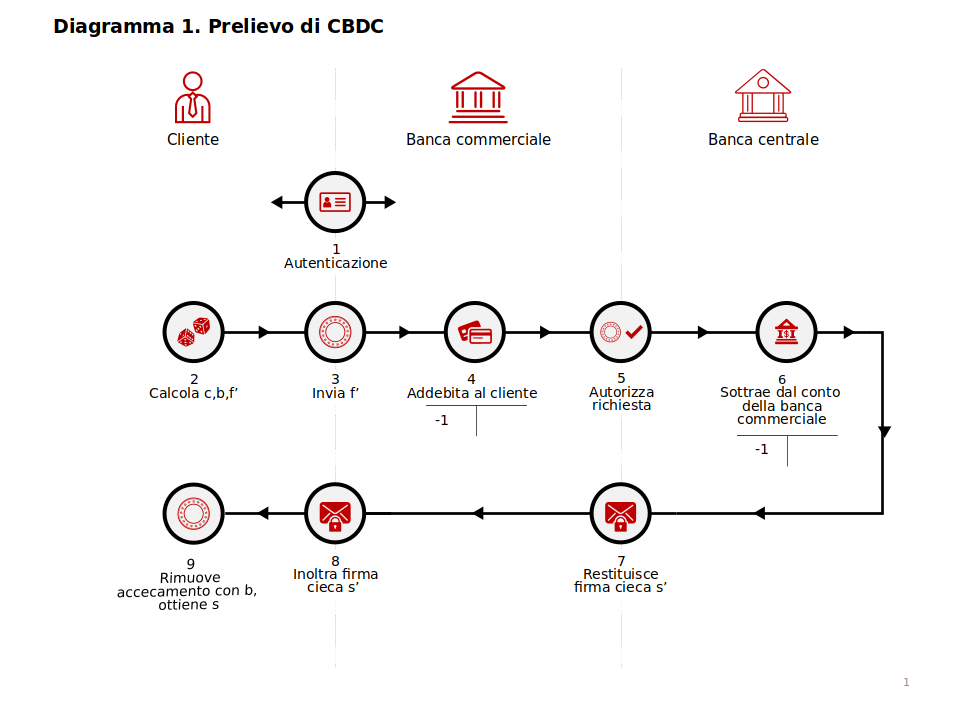
\includegraphics[width=\textwidth]{diagramma1-it.png}
  \caption{Prelievo di CBDC}
  \label{fig:fig1}
\end{figure}

Il cliente (1) invia i dati di accesso alla propria banca commerciale
utilizzando le relative procedure di autenticazione e autorizzazione.
Quindi il telefono (o il computer) del cliente ottiene la chiave di
valore pubblica $(e, n)$ fornita dalla banca centrale per quel valore; (2)
calcola quindi una coppia di chiavi per la moneta, con una chiave
privata $c$ e una chiave pubblica $C$, e sceglie un fattore di accecamento
$b$. La chiave pubblica della moneta viene quindi sottoposta a hash
($\to$ $f$) e accecata ($\to$ $f'$). Quindi il dispositivo del cliente (3)
invia $f'$ insieme all'autorizzazione a prelevare la moneta e ad
addebitarla dal conto del cliente presso la banca commerciale tramite un
canale sicuro stabilito. La banca commerciale (4) addebita quindi
l'importo dal conto deposito del cliente, (5) autorizza digitalmente la
richiesta utilizzando la firma digitale specifica della propria filiale
e inoltra la richiesta e la moneta accecata alla banca centrale per la
firma. La banca centrale (6) sottrae il valore della moneta dal conto
della banca commerciale, appone la firma cieca sulla moneta
utilizzando la chiave privata che detiene per il relativo valore e (7)
restituisce la firma cieca $s'$ alla banca commerciale. La banca
commerciale (8) inoltra la firma cieca $s'$ al portafoglio elettronico
del cliente. Infine, il dispositivo del cliente (9) utilizza $b$ per
rimuovere l'accecamento dalla firma ($\to$ $f$) e salva la moneta appena
coniata $(c, s)$.

Per spendere CBDC, la procedura è analoga al pagamento in contanti.
Tuttavia, per consolidare la transazione, il venditore deve depositare
la moneta. La procedura per spendere CBDC è illustrata nel diagramma 2.

\begin{figure}[h!]
  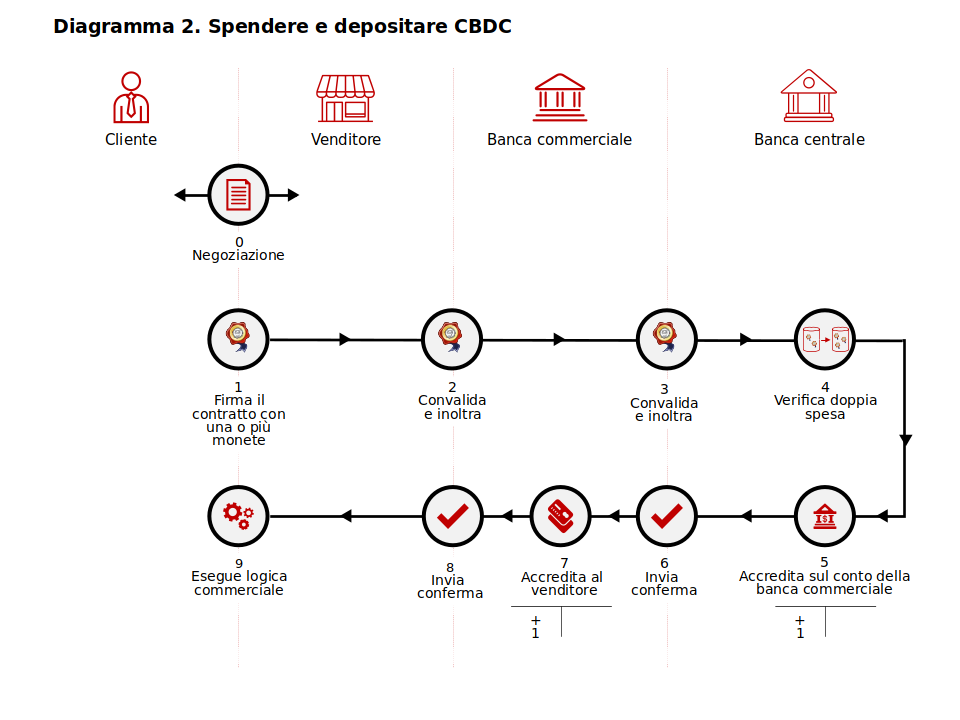
\includegraphics[width=\textwidth]{diagramma2-it.png}
  \caption{Spendere e depositare CBDC}
  \label{fig:fig2}
\end{figure}

Un cliente e un venditore negoziano un contratto commerciale. Il
cliente (1) utilizza una moneta elettronica per firmare il contratto o
l'atto di vendita con la chiave privata $c$ della moneta e trasmette la
firma al venditore. La firma di una moneta su un contratto con una
moneta valida è l'istruzione del cliente di pagare il venditore, che è
identificato dal conto bancario nel contratto. Se una singola moneta
non fosse sufficiente per coprire l'importo totale, i clienti possono
firmare il contratto con più monete. Il venditore (2) convalida quindi
la firma della moneta sul contratto e la firma $s$ della banca centrale
su $f$, che  corrisponde a quella della moneta $C$ con le rispettive
chiavi pubbliche, e inoltra la moneta firmata (insieme alle
informazioni sul conto del venditore) alla banca commerciale del
venditore. La banca commerciale del venditore (3) conferma che il
venditore è un suo cliente e inoltra la moneta firmata alla banca
centrale. La banca centrale (4) verifica le firme e controlla il
proprio database per accertarsi che la moneta non sia già stata spesa.
Se tutto è in ordine, la banca centrale (5) aggiunge la moneta
all'elenco delle monete spese, l'accredita sul conto della banca
commerciale presso la banca centrale e (6) invia una conferma in tal
senso alla banca commerciale. Quindi la banca commerciale (7)
accredita la moneta sul conto del venditore e (8) gli invia una
notifica. Il venditore (9) consegna il prodotto o servizio al cliente.
L'intera operazione richiede poche centinaia di millisecondi.

\hypertarget{considerazioni-sulla-sicurezza}{%
\subsection{Considerazioni sulla sicurezza}
\label{considerazioni-sulla-sicurezza}}

Nella nostra proposta, occorre che la banca centrale gestisca un
database e un servizio online ad alta disponibilità. Poiché le monete
elettroniche possono essere copiate dagli utenti, solo con i controlli
online si può prevenire in modo efficace la doppia spesa. Sebbene
nella teoria esistano soluzioni per identificare a posteriori gli
utenti che effettuano una doppia spesa~\cite[vedi][]{Chaum1990},
queste soluzioni creano rischi economici sia per gli utenti che per la
banca centrale a causa del ritardo nell'identificazione di
transazioni fraudolente. Il rilevamento online della doppia spesa
elimina questo rischio, ma significa anche che sarà impossibile
effettuare le transazioni se la connessione Internet alla banca
centrale non è disponibile.

La banca centrale dovrà anche proteggere la riservatezza delle chiavi
private che utilizza per firmare le monete e altri messaggi di
protocollo. Se le chiavi di firma della banca centrale dovessero
essere compromesse, ad esempio da un computer quantistico, da un
attacco fisico ai \textit{datacenter} o anche da qualche nuovo algoritmo
% FIXME:
% forme alternative:
% 1) "rimborsare AGLI utenti ... tutte le monete non spese"
% 2) "rimborsare gli utenti ... DI tutte le monete non spese"
%FIXED
imprevisto, è possibile rimborsare agli utenti --- in tutta sicurezza e
senza compromettere la privacy --- tutte le monete non spese. La banca
centrale annuncerebbe la revoca della chiave tramite l'\textit{Application
Programming Interface} (API), che verrebbe rilevata dai portafogli,
avviando quindi il seguente protocollo di aggiornamento: l'utente
svela alla banca centrale la chiave pubblica $C$ della moneta, la firma
$s$ della banca centrale e il fattore di accecamento $b$, consentendo così
alla banca centrale di verificare il legittimo prelievo dell'utente e
di rimborsare il valore della moneta non spesa. Per rilevare una
possibile compromissione della propria chiave, la banca centrale può
monitorare il database in cerca di depositi che eccedano i prelievi.

\subsection{Scalabilità e costi}\label{scalabilità-e-costi}

Lo schema che proponiamo sarebbe efficiente ed economico quanto i
moderni sistemi RTGS attualmente utilizzati dalle banche centrali.

La scalabilità si riferisce al costo di aumentare la potenza di
calcolo in modo che si possa concludere un numero crescente di
transazioni in tempi adeguati. Il costo complessivo del sistema può
essere basso in quanto la CBDC qui proposta si basa interamente su
software. Le monete spese devono essere conservate fino alla scadenza
della coppia di chiavi di valore utilizzata per firmare le monete, ad
esempio tramite un ciclo annuale continuo, che mantiene limitata la
dimensione del database. La potenza di calcolo e la larghezza di banda
necessarie aumentano della stessa quantità per ogni transazione, spesa
o deposito addizionali, dato che le transazioni sono intrinsecamente
indipendenti l'una dall'altra. Questa ulteriore potenza si ottiene
semplicemente aggiungendo più hardware, una pratica spesso conosciuta
come partizionamento o \textit{sharding}. Grazie al cosiddetto
\textit{consistent hashing}, le aggiunte di hardware non risultano
dirompenti. Si può anche utilizzare qualsiasi tipo di database.

Più nello specifico, la logica del \textit{front-end} presso la banca
centrale deve solo eseguire poche operazioni di firma, e un singolo
processore può eseguirne alcune migliaia al secondo~\cite[vedi][]{Bernstein2020}.
Se un unico sistema non fosse sufficiente, è facile aggiungere altri
server \textit{front-end} e invitare le varie banche commerciali a
bilanciare le loro richieste nella \textit{server farm} o
utilizzare un sistema di bilanciamento del carico per distribuire le
richieste all'interno dell'infrastruttura della banca centrale.

I server \textit{front-end} devono comunicare con un database per
effettuare le transazioni e prevenire la doppia spesa. Un unico server
di database moderno dovrebbe essere in grado di gestire in modo
affidabile decine di migliaia di operazioni al secondo. Le operazioni
possono essere facilmente distribuite su più server di database
semplicemente assegnando a ciascuno un intervallo di valori da
gestire. Tale configurazione garantisce che le singole transazioni non
incrocino mai le partizioni. Pertanto, anche i sistemi \textit{back-end}
dovrebbero scalare in modo lineare con le risorse di calcolo messe a
disposizione, partendo sempre da una solida base di riferimento per un
singolo sistema.

I \textit{front-end} devono anche comunicare con i \textit{back-end} per
mezzo di un'interconnessione. Queste interconnessioni possono
supportare un gran numero di transazioni al secondo. La dimensione di
una singola transazione è in genere di circa 1–10 kilobyte. Pertanto,
i \textit{datacenter} di oggi, che scambiano informazioni a 400 Gbit/s,
possono supportare milioni di transazioni al secondo.

%FIXME:
%
% Sotto appare "Probabilmente + congiuntivo".  Suggerirei
% di cambiarlo con una forma all'indicativo.  Qui si trova
% una discussione a riguardo:
% https://italian.stackexchange.com/questions/3653/probabilmente-indicativo-o-congiuntivo
% Not incorrect but FIXED anyway.
Infine, il costo totale del sistema è basso. Probabilmente il costo
principale è rappresentato dall'archiviazione sicura per
molti anni di 1–10 kilobyte per transazione. Gli esperimenti su un
prototipo di GNU Taler che utilizzava i prezzi di \textit{Amazon Web Service}
hanno stabilito che il costo del sistema (archiviazione, larghezza di
banda e capacità di calcolo) su larga scala sarebbe inferiore a
0,0001 USD per transazione~\cite[per i dettagli sui dati, si veda][]{Dold}.

\section{Considerazioni normative e politiche}
    \label{5.-considerazioni-normative-e-politiche}

Nella soluzione che proponiamo, la banca centrale non conosce
l'identità dei consumatori o dei venditori né l'importo totale delle
transazioni, ma vede solo il momento in cui le monete elettroniche vengono
rilasciate e quando vengono riscattate. Le banche commerciali continuano a
fornire l'autenticazione cruciale di consumatori e venditori e, in particolare,
custodiscono le informazioni che acquisiscono per la conoscenza dei clienti
(KYC). Le banche commerciali osservano quando i venditori ricevono fondi e, se
necessario, possono limitare la quantità di CBDC per transazione che
un singolo venditore può ricevere. Inoltre, le transazioni sono
collegate ai relativi contratti con i clienti. La conseguente
trasparenza del reddito  consente al sistema di soddisfare i requisiti
delle normative sulla lotta al riciclaggio di denaro e al
finanziamento del terrorismo (AML e CFT). In caso vengano rilevate
anomalie nei redditi dei venditori, la banca commerciale e
l'autorità fiscale o giudiziaria possono ottenere e ispezionare i
contratti relativi ai pagamenti sospetti al fine di verificarne la
legittimità. La trasparenza del reddito risultante è anche una forte
misura contro l'evasione fiscale perché i venditori non possono
sottodichiarare il proprio reddito o evadere le tasse sulle vendite.
Nel complesso, il sistema implementa gli approcci \textit{privacy-by-
design} e \textit{privacy-by-default} (come richiesto, ad esempio,
dal Regolamento generale sulla protezione dei dati dell'UE, GDPR). I
venditori non apprendono necessariamente l'identità dei propri clienti,
le banche possiedono solo le informazioni necessarie sulle attività dei
propri clienti e la banca centrale non ha accesso ai dettagli sulle
attività dei cittadini.

In alcuni paesi le normative impongono limiti per i prelievi e i
pagamenti in contanti. Tali restrizioni possono essere implementate
anche per la CBDC nel progetto proposto. Ad esempio, è possibile
stabilire una soglia per l'importo giornaliero che i consumatori possono
prelevare, oppure limitare l'importo totale di CBDC che le banche
commerciali possono convertire.

La disintermediazione del settore bancario è uno dei rischi di
instabilità finanziaria spesso sollevato per quanto riguarda la CBDC
al dettaglio. In particolare, una CBDC al dettaglio potrebbe
facilitare l'accumulo di ingenti somme di denaro della banca
centrale, il che potrebbe avere un impatto negativo sul finanziamento
alle banche mediante depositi perché il pubblico deterrebbe meno
denaro sotto forma di depositi bancari. Per i paesi le cui valute
fungono da valute rifugio, ciò potrebbe anche portare ad un aumento
degli afflussi di capitali durante i periodi globali di avversione al
rischio, dando luogo ad ulteriori pressioni sui tassi di cambio.
Quello che quindi potrebbe rappresentare un serio problema nel caso di
una CBDC basata su conti, lo sarebbe molto meno con una CBDC basata
su token. Innanzitutto, l'accumulo di una CBDC basata su token comporta
rischi di furto o perdita simili a quelli legati all'accumulo di
contanti. Tenere poche centinaia di dollari su uno smartphone è
probabilmente un rischio accettabile per molti, ma detenere una somma
molto alta è probabilmente un rischio meno accettabile. Pertanto, non
ci aspettiamo un accaparramento significativamente maggiore rispetto a
quello del denaro fisico.

Tuttavia, se l'accumulo o la massiccia conversione dei depositi
bancari in CBDC dovessero destare proccupazione, la banca centrale
avrebbe diverse opzioni. Come si è spiegato, secondo il progetto
proposto le banche centrali fissano una data di scadenza per tutte le
chiavi di firma, il che implica che in una data prestabilita le monete
firmate con quelle chiavi diventano non valide. Alla scadenza delle
chiavi di valore, i consumatori devono scambiare con monete nuove le
monete che erano state firmate con le vecchie chiavi; l'autorità di
regolamentazione può facilmente fissare una soglia di conversione per
cliente per creare un limite rigido alla quantità di CBDC che ogni
individuo può accumulare. Inoltre, la banca centrale potrebbe addebitare
commissioni, se necessario. Una commissione di aggiornamento quando le monete
stanno per scadere significherebbe nella pratica tassi di interesse negativi
sulla CBDC per limitare il suo fascino come riserva di valore, come
suggerisce~\cite{Bindseil}. Si tratterebbe infatti della diretta attuazione
dell'idea di Silvio Gesell di applicare una tassa di possesso sulla moneta,
notoriamente citata da~\cite{Keynes} e ripresa da~\cite{Goodfriend},
\cite{Buiter} e~\cite{Agarwal}.

Per quanto riguarda le implicazioni in termini di politica monetaria,
non dovrebbero esserci cambiamenti reali perché la nostra CBDC è
progettata per replicare il contante piuttosto che i depositi bancari.
L'emissione, il prelievo e il deposito della nostra CBDC corrispondono
esattamente all'emissione, al prelievo e al deposito di banconote. È
possibile che la velocità di circolazione di una CBDC al dettaglio sia
diversa da quella del contante fisico, ma questo non dovrebbe
rappresentare un problema significativo per la politica monetaria.

\hypertarget{lavori-correlati}{%
\section{Lavori correlati}\label{6.-lavori-correlati}}

Come segnalato in precedenza, la CBDC che si propone in questo documento
si basa su eCash e GNU Taler.\footnote{L'implementazione di eCash
da parte della società DigiCash negli anni novanta è documentata su
\url{https://www.chaum.com/ecash}.} A partire dalla proposta originale
e-Cash di Chaum, la ricerca si è concentrata su tre questioni principali.
In primo luogo, nella proposta originale di Chaum le monete avevano un
valore fisso e potevano essere spese solo nella loro totalità. Pagare
grandi somme con monete denominate in centesimi sarebbe stato poco
efficiente; quindi~\cite{Okamoto}, \cite{Camenisch2005}, \cite{Canard}
e~\cite{Dold} idearono modi per affrontare il problema. Queste soluzioni
comprendono protocolli per dare il resto o rendere divisibili le monete.

Un secondo problema riguarda gli errori nelle transazioni dovuti ad
interruzioni della rete. In questo caso, il sistema deve garantire che
i fondi rimangano in possesso del consumatore senza pregiudicare la
privacy. L'\textit{Endorsed E-Cash} proposto da~\cite{Camenisch2007},
così come da~\cite{Dold}, affrontano entrambi questo problema. Molte
delle soluzioni violano le garanzie sulla privacy per i clienti che
utilizzano queste funzionalità e tutte, tranne Taler, violano il
requisito della trasparenza del reddito.

La terza questione importante, spesso trascurata, è la trasparenza del
reddito e quindi la conformità con i requisiti AML e KYC. \cite{Fuchsbauer}
hanno deliberatamente progettato il loro sistema di disintermediazione
per fornire una semantica più simile al contante. Tuttavia, la
disintermediazione totale è in genere difficile da concialiare con le
normative AML e KYC dato che diventa impossibile raggiungere qualsiasi
livello di responsabilità. Un esempio di tale architettura è ZCash, un
registro distribuito (\textit{ledger}) che nasconde dalla rete le
informazioni sul pagatore, sul beneficiario e sull'importo della
transazione, rendendolo quindi il sistema di pagamento perfetto per la
criminalità online. Solo Taler offre sia una privacy costante per i
clienti che la trasparenza del reddito, fornendo al contempo un sistema
di resto efficiente, scambi atomici~\cite[vedi][]{Camenisch2007} e la
possibilità di ripristinare i portafogli dal backup.

Per quanto riguarda i sistemi di pagamento per le CBDC, \cite{Danezis}
hanno progettato un \textit{ledger} scalabile per RSCoin. Si tratta
fondamentalmente di un sistema RTGS che viene protetto utilizzando la
stessa crittografia che si usa in Bitcoin. Come Taler, il design utilizza
lo \textit{sharding} del database per consentire la scalabilità lineare.
Tuttavia, la soluzione di Danezis e Meiklejohn non prevede alcuna
disposizione per la privacy e manca di elementi per l'integrazione
pratica del design con i sistemi e i processi bancari esistenti.

L'EUROchain della Banca Centrale Europea\cite[vedi][]{ECB} è un altro
prototipo di CBDC con registro distribuito. Simile all'architettura
proposta in questo documento, EUROchain utilizza un'architettura a due
livelli in cui le banche commerciali agiscono come intermediari. Una
differenza cruciale è il modo in cui i sistemi cercano di combinare
privacy e conformità con la normativa antiriciclaggio (AML). Mentre nel
nostro progetto l'autorità di regolamentazione può imporre un limite
alla somma di denaro elettronico che un titolare di conto bancario può
prelevare in un determinato periodo di tempo, EUROchain emette un numero
limitato di «voucher di anonimato» che garantiscono al destinatario un
numero limitato di transazioni senza controlli AML. Poiché questi voucher
sembrano essere privi di qualsiasi token di valore, non è chiaro come
il design possa impedire l'emergere di un mercato nero per i «voucher
di anonimato». Inoltre, la nozione di anonimato di EUROchain è molto
diversa, in quanto i loro «voucher di anonimato» eliminano solo alcuni
controlli AML, preservando la capacità delle banche commerciali di
sapere in che modo i clienti spendono il denaro elettronico. Laddove chi
paga utilizzando Taler interagisce direttamente con i venditori per
spendere il proprio contante elettronico, il sistema EUROchain chiede
ai pagatori di istruire le proprie banche commerciali per accedere alle
CBDC. Pertanto, EUROchain non emette direttamente token di valore ai
consumatori, affida invece ai consumatori il compito di autenticarsi
presso la propria banca commerciale per accedere alle CBDC che la
banca centrale detiene effettivamente in deposito a garanzia. Non è
quindi evidente quali siano i vantaggi di EUROchain in termini di
privacy, prestazioni o sicurezza rispetto all'attuale denaro in deposito.

\section{Conclusione}\label{7.-conclusione}

Con l'emergere di Bitcoin e valute digitali come Diem (già nota come
Libra) recentemente proposte dai colossi del web, le banche centrali
affrontano una crescente concorrenza da parte di operatori privati che
offrono la propria alternativa digitale al contante fisico. Le decisioni
delle banche centrali sull'emissione o meno di una CBDC dipendono dalla
loro valutazione dei benefici e dei rischi di una CBDC. È probabile che
questi vantaggi e rischi, nonché le circostanze giurisdizionali
specifiche che definiscono l'ambito di applicazione di una CBDC al
dettaglio, differiscano da un paese all'altro.

Se una banca centrale decide di emettere una CBDC al dettaglio,
proponiamo una CBDC basata su token che combina la privacy delle
transazioni con la conformità alle normative KYC, AML e CFT. Tale CBDC
non sarebbe in concorrenza con i depositi presso le banche commerciali,
replicherebbe piuttosto il contante fisico, limitando quindi i rischi di
stabilità finanziaria e di perturbazione della politica monetaria.

Abbiamo dimostrato che lo schema qui proposto sarebbe efficiente ed
economico quanto i moderni sistemi RTGS gestiti dalle banche centrali.
I pagamenti elettronici con la nostra CBDC richiederebbero solo un
semplice database e minuscole quantità di larghezza di banda per le
transazioni. L'efficienza e l'economicità di questa soluzione, insieme
alla maggiore facilità d'uso da parte del consumatore determinata dal
passaggio dall'autenticazione all'autorizzazione, rendono questo schema
probabilmente il primo a supportare l'annoso obiettivo dei micropagamenti
online. Inoltre, l'uso di monete per firmare crittograficamente contratti
elettronici consente anche l'impiego di contratti intelligenti. Ciò
potrebbe anche portare all'emergere di applicazioni completamente nuove
per i sistemi di pagamento. Sebbene il nostro sistema non sia basato su
DLT, può essere facilmente integrato con tali tecnologie se richiesto
dalle future infrastrutture del mercato finanziario.

Altrettanto importante, una CBDC al dettaglio deve rimanere, come il
contante fisico, un bene rispettoso della privacy sotto il controllo
individuale dei cittadini. Lo schema proposto in questo studio soddisfa
questo criterio e consente alle banche centrali di evitare gravi sfide
alla loro politica monetaria e alla stabilità finanziaria sfruttando al
contempo i vantaggi del passaggio al digitale.

\newpage
\bibliographystyle{agsm}
\bibliography{cbdc-it}

\end{document}
